% Options for packages loaded elsewhere
\PassOptionsToPackage{unicode}{hyperref}
\PassOptionsToPackage{hyphens}{url}
\PassOptionsToPackage{dvipsnames,svgnames,x11names}{xcolor}
%
\documentclass[
  12pt,
]{article}

\usepackage{amsmath,amssymb}
\usepackage{setspace}
\usepackage{iftex}
\ifPDFTeX
  \usepackage[T1]{fontenc}
  \usepackage[utf8]{inputenc}
  \usepackage{textcomp} % provide euro and other symbols
\else % if luatex or xetex
  \usepackage{unicode-math}
  \defaultfontfeatures{Scale=MatchLowercase}
  \defaultfontfeatures[\rmfamily]{Ligatures=TeX,Scale=1}
\fi
\usepackage{lmodern}
\ifPDFTeX\else  
    % xetex/luatex font selection
\fi
% Use upquote if available, for straight quotes in verbatim environments
\IfFileExists{upquote.sty}{\usepackage{upquote}}{}
\IfFileExists{microtype.sty}{% use microtype if available
  \usepackage[]{microtype}
  \UseMicrotypeSet[protrusion]{basicmath} % disable protrusion for tt fonts
}{}
\makeatletter
\@ifundefined{KOMAClassName}{% if non-KOMA class
  \IfFileExists{parskip.sty}{%
    \usepackage{parskip}
  }{% else
    \setlength{\parindent}{0pt}
    \setlength{\parskip}{6pt plus 2pt minus 1pt}}
}{% if KOMA class
  \KOMAoptions{parskip=half}}
\makeatother
\usepackage{xcolor}
\setlength{\emergencystretch}{3em} % prevent overfull lines
\setcounter{secnumdepth}{5}
% Make \paragraph and \subparagraph free-standing
\makeatletter
\ifx\paragraph\undefined\else
  \let\oldparagraph\paragraph
  \renewcommand{\paragraph}{
    \@ifstar
      \xxxParagraphStar
      \xxxParagraphNoStar
  }
  \newcommand{\xxxParagraphStar}[1]{\oldparagraph*{#1}\mbox{}}
  \newcommand{\xxxParagraphNoStar}[1]{\oldparagraph{#1}\mbox{}}
\fi
\ifx\subparagraph\undefined\else
  \let\oldsubparagraph\subparagraph
  \renewcommand{\subparagraph}{
    \@ifstar
      \xxxSubParagraphStar
      \xxxSubParagraphNoStar
  }
  \newcommand{\xxxSubParagraphStar}[1]{\oldsubparagraph*{#1}\mbox{}}
  \newcommand{\xxxSubParagraphNoStar}[1]{\oldsubparagraph{#1}\mbox{}}
\fi
\makeatother


\providecommand{\tightlist}{%
  \setlength{\itemsep}{0pt}\setlength{\parskip}{0pt}}\usepackage{longtable,booktabs,array}
\usepackage{calc} % for calculating minipage widths
% Correct order of tables after \paragraph or \subparagraph
\usepackage{etoolbox}
\makeatletter
\patchcmd\longtable{\par}{\if@noskipsec\mbox{}\fi\par}{}{}
\makeatother
% Allow footnotes in longtable head/foot
\IfFileExists{footnotehyper.sty}{\usepackage{footnotehyper}}{\usepackage{footnote}}
\makesavenoteenv{longtable}
\usepackage{graphicx}
\makeatletter
\newsavebox\pandoc@box
\newcommand*\pandocbounded[1]{% scales image to fit in text height/width
  \sbox\pandoc@box{#1}%
  \Gscale@div\@tempa{\textheight}{\dimexpr\ht\pandoc@box+\dp\pandoc@box\relax}%
  \Gscale@div\@tempb{\linewidth}{\wd\pandoc@box}%
  \ifdim\@tempb\p@<\@tempa\p@\let\@tempa\@tempb\fi% select the smaller of both
  \ifdim\@tempa\p@<\p@\scalebox{\@tempa}{\usebox\pandoc@box}%
  \else\usebox{\pandoc@box}%
  \fi%
}
% Set default figure placement to htbp
\def\fps@figure{htbp}
\makeatother
% definitions for citeproc citations
\NewDocumentCommand\citeproctext{}{}
\NewDocumentCommand\citeproc{mm}{%
  \begingroup\def\citeproctext{#2}\cite{#1}\endgroup}
\makeatletter
 % allow citations to break across lines
 \let\@cite@ofmt\@firstofone
 % avoid brackets around text for \cite:
 \def\@biblabel#1{}
 \def\@cite#1#2{{#1\if@tempswa , #2\fi}}
\makeatother
\newlength{\cslhangindent}
\setlength{\cslhangindent}{1.5em}
\newlength{\csllabelwidth}
\setlength{\csllabelwidth}{3em}
\newenvironment{CSLReferences}[2] % #1 hanging-indent, #2 entry-spacing
 {\begin{list}{}{%
  \setlength{\itemindent}{0pt}
  \setlength{\leftmargin}{0pt}
  \setlength{\parsep}{0pt}
  % turn on hanging indent if param 1 is 1
  \ifodd #1
   \setlength{\leftmargin}{\cslhangindent}
   \setlength{\itemindent}{-1\cslhangindent}
  \fi
  % set entry spacing
  \setlength{\itemsep}{#2\baselineskip}}}
 {\end{list}}
\usepackage{calc}
\newcommand{\CSLBlock}[1]{\hfill\break\parbox[t]{\linewidth}{\strut\ignorespaces#1\strut}}
\newcommand{\CSLLeftMargin}[1]{\parbox[t]{\csllabelwidth}{\strut#1\strut}}
\newcommand{\CSLRightInline}[1]{\parbox[t]{\linewidth - \csllabelwidth}{\strut#1\strut}}
\newcommand{\CSLIndent}[1]{\hspace{\cslhangindent}#1}

\usepackage{graphicx}
\usepackage{float}
\setlength{\parindent}{2em}
\usepackage[margin=1in]{geometry}
\makeatletter
\@ifpackageloaded{tcolorbox}{}{\usepackage[skins,breakable]{tcolorbox}}
\@ifpackageloaded{fontawesome5}{}{\usepackage{fontawesome5}}
\definecolor{quarto-callout-color}{HTML}{909090}
\definecolor{quarto-callout-note-color}{HTML}{0758E5}
\definecolor{quarto-callout-important-color}{HTML}{CC1914}
\definecolor{quarto-callout-warning-color}{HTML}{EB9113}
\definecolor{quarto-callout-tip-color}{HTML}{00A047}
\definecolor{quarto-callout-caution-color}{HTML}{FC5300}
\definecolor{quarto-callout-color-frame}{HTML}{acacac}
\definecolor{quarto-callout-note-color-frame}{HTML}{4582ec}
\definecolor{quarto-callout-important-color-frame}{HTML}{d9534f}
\definecolor{quarto-callout-warning-color-frame}{HTML}{f0ad4e}
\definecolor{quarto-callout-tip-color-frame}{HTML}{02b875}
\definecolor{quarto-callout-caution-color-frame}{HTML}{fd7e14}
\makeatother
\makeatletter
\@ifpackageloaded{caption}{}{\usepackage{caption}}
\AtBeginDocument{%
\ifdefined\contentsname
  \renewcommand*\contentsname{Table of contents}
\else
  \newcommand\contentsname{Table of contents}
\fi
\ifdefined\listfigurename
  \renewcommand*\listfigurename{List of Figures}
\else
  \newcommand\listfigurename{List of Figures}
\fi
\ifdefined\listtablename
  \renewcommand*\listtablename{List of Tables}
\else
  \newcommand\listtablename{List of Tables}
\fi
\ifdefined\figurename
  \renewcommand*\figurename{Figure}
\else
  \newcommand\figurename{Figure}
\fi
\ifdefined\tablename
  \renewcommand*\tablename{Table}
\else
  \newcommand\tablename{Table}
\fi
}
\@ifpackageloaded{float}{}{\usepackage{float}}
\floatstyle{ruled}
\@ifundefined{c@chapter}{\newfloat{codelisting}{h}{lop}}{\newfloat{codelisting}{h}{lop}[chapter]}
\floatname{codelisting}{Listing}
\newcommand*\listoflistings{\listof{codelisting}{List of Listings}}
\usepackage{amsthm}
\theoremstyle{plain}
\newtheorem{theorem}{Theorem}[section]
\theoremstyle{remark}
\AtBeginDocument{\renewcommand*{\proofname}{Proof}}
\newtheorem*{remark}{Remark}
\newtheorem*{solution}{Solution}
\newtheorem{refremark}{Remark}[section]
\newtheorem{refsolution}{Solution}[section]
\makeatother
\makeatletter
\makeatother
\makeatletter
\@ifpackageloaded{caption}{}{\usepackage{caption}}
\@ifpackageloaded{subcaption}{}{\usepackage{subcaption}}
\makeatother
\makeatletter
\@ifpackageloaded{tcolorbox}{}{\usepackage[skins,breakable]{tcolorbox}}
\makeatother
\makeatletter
\@ifundefined{shadecolor}{\definecolor{shadecolor}{rgb}{.97, .97, .97}}{}
\makeatother
\makeatletter
\makeatother
\makeatletter
\ifdefined\Shaded\renewenvironment{Shaded}{\begin{tcolorbox}[breakable, boxrule=0pt, frame hidden, sharp corners, interior hidden, enhanced]}{\end{tcolorbox}}\fi
\makeatother

\usepackage{bookmark}

\IfFileExists{xurl.sty}{\usepackage{xurl}}{} % add URL line breaks if available
\urlstyle{same} % disable monospaced font for URLs
\hypersetup{
  pdftitle={What a Generative Models?},
  pdfauthor={Yuyang Zhang},
  colorlinks=true,
  linkcolor={blue},
  filecolor={Maroon},
  citecolor={Blue},
  urlcolor={Blue},
  pdfcreator={LaTeX via pandoc}}


\title{\textbf{What a Generative Models?}}
\author{Yuyang Zhang}
\date{2025-04-30}

\begin{document}
\maketitle

\renewcommand*\contentsname{Contents}
{
\hypersetup{linkcolor=}
\setcounter{tocdepth}{2}
\tableofcontents
}

\setstretch{1.3}
\section{What is the Generative Models and Generative
AI?}\label{what-is-the-generative-models-and-generative-ai}

Generative models, as the name indicated, are models that can
\emph{generative} new content. Unlike \textbf{discriminate models}, the
generative models are sometime hard to train. But why we need generative
models in the first place? We want generative models because:

\begin{itemize}
\tightlist
\item
  \href{https://en.wikipedia.org/wiki/Density_estimation}{Density
  Estimation}: Estimate the probability density function of the data.
\item
  \href{https://en.wikipedia.org/wiki/Anomaly_detection}{Anomaly
  Detection}: Detect the anomaly data points.
\item
  \href{https://en.wikipedia.org/wiki/Imputation}{Imputation}: Fill in
  the missing data.
\item
  \href{https://en.wikipedia.org/wiki/Data_augmentation}{Data
  Augmentation}: Generate new data to increase the size of the dataset.
\item
  \href{https://en.wikipedia.org/wiki/Data_generation}{Data Generation}:
  Generate new data to train the model.
\item
  \href{https://en.wikipedia.org/wiki/Data_compression}{Data
  Compression}: Compress the data to save the storage.
\item
  \href{https://en.wikipedia.org/wiki/Denoising}{Data Denoising}: Remove
  the noise from the data.
\item
  \href{https://en.wikipedia.org/wiki/Latent_space}{Latent Space
  Exploration}: Explore the latent space of the data.
\item
  \href{https://en.wikipedia.org/wiki/Interpolation}{Latent Space
  Interpolation}: Interpolate between the data points.
\end{itemize}

\begin{figure}

\centering{

\pandocbounded{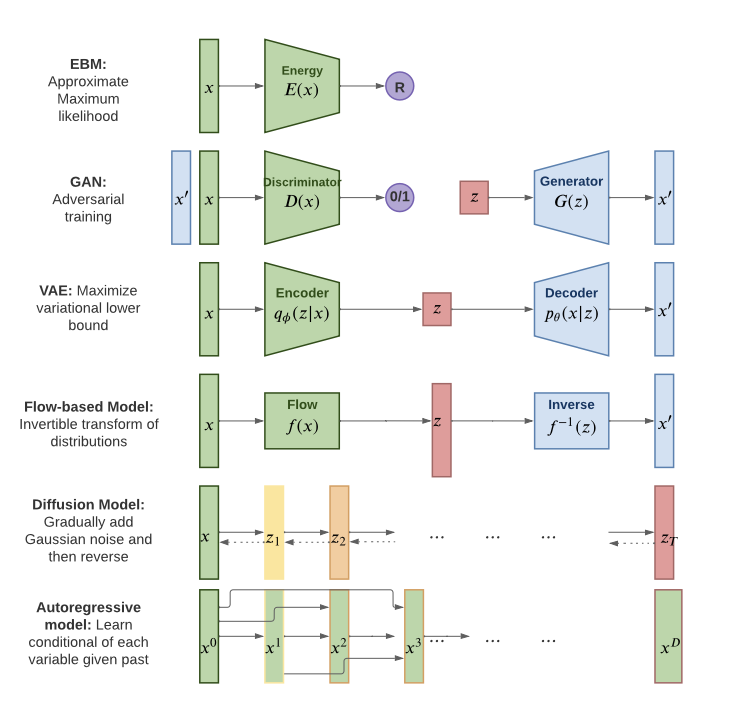
\includegraphics[keepaspectratio]{Generative Model Overview_files/mediabag/202503062129654.png}}

}

\caption{\label{fig-overview-generative-models}Summary of various kinds
of deep generative models. (Image Source: Probabilistic Machine
Learning)}

\end{figure}%

Generative Models can solve \textbf{inverse problems}. For example, the
medical image reconstruction. Herea re some example of the generative
models in the real world:

\begin{itemize}
\tightlist
\item
  Text to Image Model: this is common in the current AI, for example,
  the Stable Diffusion Model and Dalles model, below are the example of
  the generation of Chat-4o model:
\end{itemize}

\begin{figure}

\centering{

\pandocbounded{
\includegraphics[keepaspectratio]{images/paste-5.png}}

}

\caption{\label{fig-text2img-wine-glass}Image Generation through
ChatGPT-4o model.}

\end{figure}%

\begin{itemize}
\tightlist
\item
  Text to Video model such as Sora.
\end{itemize}

\begin{figure}

\centering{

\url{images/sora-generation.mp4}

}

\caption{\label{fig-cern}}

\end{figure}%

In the blog, we will learn three things:

\begin{itemize}
\tightlist
\item
  Representation: how to model the joint distribution of many random
  variables
\item
  Learning: how to learn and compare the different probability
  distribution
\item
  Inference: how to invert the generation process ( recover high-level
  description (latent variables) from raw data(images, text\ldots)
\end{itemize}

Besides the three main topics, we will introduce 6 different generative
models as showed in the Figure~\ref{fig-overview-generative-models}. In
this article, we will go through those 6 different types. Get into the
details of each different types and compare models. How to combine those
model to get more complex modeling ability.

\begin{tcolorbox}[enhanced jigsaw, toprule=.15mm, colframe=quarto-callout-note-color-frame, bottomrule=.15mm, rightrule=.15mm, colbacktitle=quarto-callout-note-color!10!white, opacitybacktitle=0.6, colback=white, arc=.35mm, bottomtitle=1mm, left=2mm, leftrule=.75mm, breakable, title=\textcolor{quarto-callout-note-color}{\faInfo}\hspace{0.5em}{Note}, titlerule=0mm, toptitle=1mm, opacityback=0, coltitle=black]

In this blog, we only going through the \emph{main ideas} of the
different models, if you want to dig into different topics more deeply,
please check my following blogs:

\begin{itemize}
\tightlist
\item
  \href{https://yyzhang2000.github.io/Blog/posts/Generative\%20Model/VAE.html}{Variational
  AutoEncoder Models}
\item
  \href{https://yyzhang2000.github.io/Blog/posts/Generative\%20Model/Diffusion\%20Model.html}{Diffusion
  Models}
\item
  Auto-Regressive Models (Coming soon\ldots)
\item
  Flow Matching(Coming soon\ldots)
\item
  GAN(Coming soon\ldots)
\end{itemize}

\end{tcolorbox}

\section{Maximum Likelihood Learning}\label{maximum-likelihood-learning}

\begin{figure}

\centering{

\pandocbounded{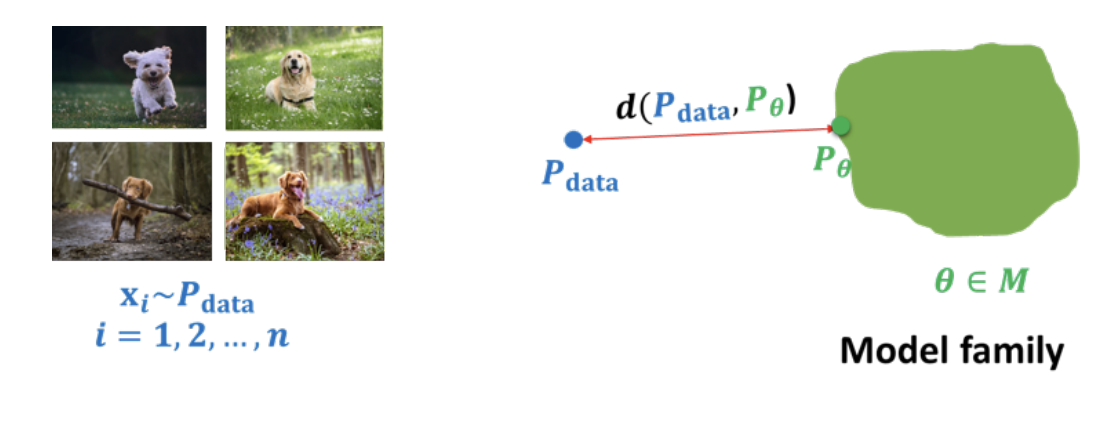
\includegraphics[keepaspectratio]{Generative Model Overview_files/mediabag/202504082033591.png}}

}

\caption{\label{fig-mle}Compare modelled distribution with true
distribution (Image Source: Stanford CS236 Deep Generative)}

\end{figure}%

The purpose of the most generative models is to learn the probability
distribution \(P_\theta\) that is close to the true distribution
\(P_\text{data}\) which we don't know. There are different form of the
\(P_\theta\), how do we choose the ``best'' model to represent the
\(P_\text{data}\). We can use the Kullback-Leibler divergence
(KL-divergence) between two distribution to measure how different those
two distributions are. The KL-Divergence is defined as:

\begin{equation}\phantomsection\label{eq-kl-divergence}{
\begin{split}D_{KL} (P\| Q ) & = \mathbb{E}_{P}\left[ \log \frac{P(x)}{Q(x)} \right]  \\& = \mathbb{E}_{P}[\log P(x)] - \mathbb{E}_{P}[\log Q(x)]\end{split}
}\end{equation}

Two of the good property of the KL-Divergence are:

\begin{itemize}
\tightlist
\item
  \(D_{KL} \geq 0\): when \(Q = P\) we can get the equal
\item
  \(\mathbb{E}_{P}\left[ - \log \frac{Q}{P} \right] \geq -\log \mathbb{E}_{P}\left[ \frac{Q}{P} \right]\):
  due to
  the\href{https://en.wikipedia.org/wiki/Jensen\%27s_inequality}{Jensen's
  inequality} and \(-\log\) is the convex function.
\end{itemize}

So, we can measure how the \(P_{\text{data}}\) and \(P_{\theta}\) are
different:

\begin{equation}\phantomsection\label{eq-kl-of-two-model-and-true}{
\begin{split}D_{KL}(P_{\text{data}} \| P_{\theta}) & = \mathbb{E}_{x \sim P_{\text{data}}} \left[ \log \frac{P_{data}(x)}{P_{\theta}(x)} \right] \\ &=   \mathbb{E}_{x \sim P_{\text{data}}} [\log P_{\text{data}}(x)] - \textcolor{green}{\mathbb{E}_{x \sim P_{\text{data}}} [\log P_{\theta}(x)]}\\\end{split}
}\end{equation}

As we can see, the first term is not related to the \(\theta\), which
means const across all the models and we don't know the value. We only
need to \textbf{maximizing} the
\(\textcolor{green}{\mathbb{E}_{x \sim P_{\text{data}}} [\log P_{\theta}(x)]}\)
in order to minimizing the \(D_{KL}\).

\begin{tcolorbox}[enhanced jigsaw, toprule=.15mm, colframe=quarto-callout-note-color-frame, bottomrule=.15mm, rightrule=.15mm, colbacktitle=quarto-callout-note-color!10!white, opacitybacktitle=0.6, colback=white, arc=.35mm, bottomtitle=1mm, left=2mm, leftrule=.75mm, breakable, title=\textcolor{quarto-callout-note-color}{\faInfo}\hspace{0.5em}{Note}, titlerule=0mm, toptitle=1mm, opacityback=0, coltitle=black]

Notes that, although we can compare models, we are still not know how
close we are to the true distribution \(P_{\text{data}}\).

\end{tcolorbox}

How to calculate
\(\mathbb{E}_{x \sim P_{\text{data}}} [\log P_{\theta}(x)]\), one way is
to approximate the expected log-likelihood with empirical
log-likelihood: \[
\mathbb{E}_{x \sim P_{\text{data}}} [\log P_{\theta}(x)] \approx \mathbb{E}_{\mathcal{D}}[\log P_{\theta}(x)]  
= \frac{1}{|\mathcal{D}|} \sum_{x \in \mathcal{D}} \log P_{\theta}(x)
\]

So, the maximum likelihood learning become: \[
\underset{P_{\theta}}{\max}  \frac{1}{|\mathcal{D}|} \sum_{x \in \mathcal{D}} \log P_{\theta}(x)
\]

The maximum of the likelihood function is equal to minimizing the
\textbf{negative log-likelihood(NLL)}: \[
\underset{P_{\theta}}{\max}  \frac{1}{|\mathcal{D}|} \sum_{x \in \mathcal{D}} \log P_{\theta}(x)   
\quad \Longleftrightarrow \quad
\underset{P_{\theta}}{\min} \frac{1}{|\mathcal{D}|} \sum_{x \in \mathcal{D}} -\log P_{\theta}(x) 
\] So, the loss function is: \[
\mathcal{L}(\theta) = \frac{1}{|\mathcal{D}|} \sum_{x \in \mathcal{D}} -\log P_{\theta}(x) 
\]

Depending on what form~ \(p_\theta(x)\)~ takes, this NLL simplifies into
familiar losses like \textbf{MSE} or \textbf{CrossEntropy}.

When translating the above mathematical formulation into code, we
commonly used some form:

\begin{itemize}
\tightlist
\item
  Mean Squared Loss (MSE): Diffusion Models
\item
  Cross-Entropy Loss: GAN(Binary Cross Entropy)
\end{itemize}

\begin{tcolorbox}[enhanced jigsaw, toprule=.15mm, colframe=quarto-callout-note-color-frame, bottomrule=.15mm, rightrule=.15mm, colbacktitle=quarto-callout-note-color!10!white, opacitybacktitle=0.6, colback=white, arc=.35mm, bottomtitle=1mm, left=2mm, leftrule=.75mm, breakable, title=\textcolor{quarto-callout-note-color}{\faInfo}\hspace{0.5em}{Why we can convert MLE to loss fucn}, titlerule=0mm, toptitle=1mm, opacityback=0, coltitle=black]

Assume the model outputs the \textbf{mean} of a Gaussian distribution:
\[p_\theta(x) = \mathcal{N}(x; \mu_\theta, \sigma^2 I)\] Then the
log-likelihood is:
\[\log p_\theta(x) = -\frac{1}{2\sigma^2} \|x - \mu_\theta\|^2 + \text{const}\]
So the \textbf{negative log-likelihood} becomes:
\[-\log p_\theta(x) = \frac{1}{2\sigma^2} \|x - \mu_\theta\|^2 + \text{const}\]

One of the problem with the MLE is that, it can easily overfit the data,
that means it might not generalize well on the un-seen data set. There
are several way to avoid the overfitting:

\begin{itemize}
\tightlist
\item
  Hard Constraints: limit the choice of the NN
\item
  Soft preference for ``Simpler'' Models
\item
  Augment the objective function with regularization
\end{itemize}

\[
\text{obj}(x, \mathcal{M}) = \text{loss}(x, \mathcal{M}) + R(\mathcal{M})
\]

\begin{itemize}
\tightlist
\item
  Evaluate generalization performance on a held-out validation set.
\end{itemize}

\end{tcolorbox}

\section{Auto-Regressive Models}\label{auto-regressive-models}

\begin{figure}

\begin{minipage}{0.50\linewidth}

\begin{figure}[H]

{\centering 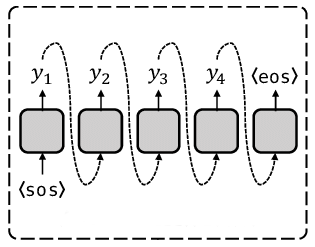
\includegraphics[width=5in,height=5.14583in]{Generative Model Overview_files/mediabag/1-PLsOLk_kmYwW59UeYh.png}

}

\subcaption{Auto-Regressive Model of Language Model}

\end{figure}%

\end{minipage}%
%
\begin{minipage}{0.50\linewidth}

\begin{figure}[H]

{\centering 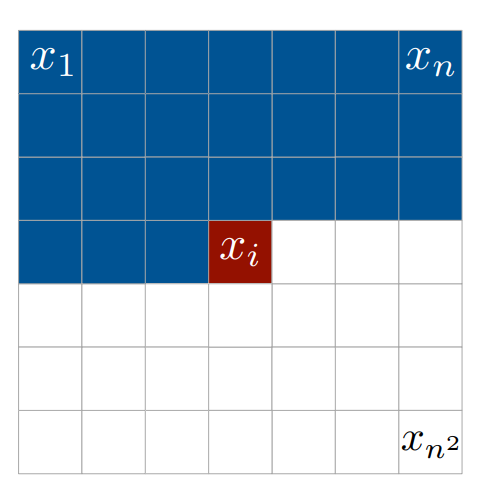
\includegraphics[width=5in,height=\textheight,keepaspectratio]{Generative Model Overview_files/mediabag/2017-02-22-183010_47.png}

}

\subcaption{PixelCNN for the Image Modeling}

\end{figure}%

\end{minipage}%

\end{figure}%

\begin{theorem}[Auto Regressive
Model]\protect\hypertarget{thm-ar}{}\label{thm-ar}

An \textbf{auto-regressive generative model} is a type of
\textbf{generative model} that models the \textbf{joint probability
distribution} of a sequence (e.g., words, pixels, audio samples) by
factorizing it into a \textbf{product of conditional
probabilities}---each conditioned on the previous elements
Mathematically, given a sequence \(x = (x_1, x_2, \cdots, x_T)\), the
joint probability is modeled as \[
P_\theta(\mathrm{x}) = \prod_{t=1}^T P_\theta(x_t | x_{<t})
\]

\end{theorem}

For more details, please check my this \href{}{blog}

\section{Variational AutoEncoder
Models}\label{variational-autoencoder-models}

For more details, please check my this
\href{https://yyzhang2000.github.io/Blog/posts/Generative\%20Model/VAE.html}{blog}

\begin{theorem}[VAE]\protect\hypertarget{thm-vae}{}\label{thm-vae}

A VAE aims to model a generative process for data \(x\) by introducing
latent variables \(z\). The key idea involves optimizing the
\textbf{Evidence Lower Bound (ELBO)}:

\[
\mathcal{L}(\theta, \phi; x) = \mathbb{E}_{q_{\phi}(z|x)}[\log p_{\theta}(x|z)] - D_{\text{KL}}\left[q_{\phi}(z|x) \| p(z)\right]
\]

where:

\begin{itemize}
\tightlist
\item
  \(p_\theta(x | z)\) is the decoder network parameterized by
  \(\theta\), often modeled as
  \(p_\theta(x | z) = \mathcal{N}(x; \mu_\theta(z), \sigma^2I)\)
\item
  \(q_\phi(z|x)\) is the approximated distribution for the true
  posterior \(p(z|x)\), this is the encoder part, modeled as:
  \(q_\phi(z | x) = \mathcal{N}(z; \mu_\phi(x), \sigma_\phi^2(x))\)
\end{itemize}

Thus the training objective for the VAE is:

\[
\max_{\theta, \phi}\; \mathbb{E}_{x \sim p_{\text{data}}(x)}[\mathcal{L}(\theta, \phi; x)]
\]

\end{theorem}

\url{https://mlarchive.com/wp-content/uploads/2022/09/New-Project-3.png}

The VAE model we are going to introduce is the Variational AutoEncoder.
The original VAE objective (ELBO) is derived from MLE.

\[
\begin{split}\log p(x) &= \log \int p(x, z) \, dz \\&= \log  \int \textcolor{green}{\frac{q(z|x)}{q(z|x)}} p(x, z) \, dz  \\&=  \log \mathbb{E}_{\textcolor{green}{q(z|x)}}\left[ \frac{p(x,z)}{\textcolor{green}{q(z|x)}} \right] \\ &\geq  \mathbb{E}_{\textcolor{green}{q(z|x)}}\left[ \log \frac{p(x,z)}{\textcolor{green}{q(z|x)}} \right]  && \text{(Jensen's Inequality)}\\ & =\underbrace{ \mathbb{E}_{\textcolor{green}{q(z|x)}}[\log p(x, z) -  \log\textcolor{green}{q(z|x)}] }_{ ELBO } \\&=  \mathbb{E}_{\textcolor{green}{q(z|x)}}[\log p(x |z) +\log p(z) - \log (\textcolor{green}{q(z |x)})] \\ &=  \mathbb{E}_{\textcolor{green}{q(z|x)}}[\log p(x|z)]   - \mathbb{E}_{\textcolor{green}{q(z|x)}}\left[ \log \frac{\textcolor{green}{q(z|x)}}{p(x)} \right] \\ &=  \mathbb{E}_{\textcolor{green}{q(z|x)}}[\log p(x|z)]  - D_{KL}(\textcolor{green}{q(z |x)} \| p(z)  ) \\\end{split}
\]

Since the \(\textcolor{green}{q(z|x)}\) is intractable because of the
high dimension, we use another function to \emph{approximate} it. Same
for the \(p(x | z)\). So, the MLE object become:

\[
\begin{align} &\max \quad  \mathbb{E}_{\textcolor{green}{q(z|x)}}[\log p(x|z)]  - D_{KL}(\textcolor{green}{q(z |x)} \| p(z)  )  \\  \implies &\min_{\theta,\phi} \quad -\mathbb{E}{q_{\phi}(z|x)}[\log p_{\theta}(x|z)] + D_{\text{KL}}(q_{\phi}(z|x)\|p(z))\end{align}
\]

The \(p(z)\) is the prior distribution of latent variable is usually as
MultiVariate Gaussian Distribution. However, we can set more fancy and
complex distribution as the prior distribution.

There are several tricks used during the training of VAE, the first one
is the reparameterization tirck.

\subsection{Reparameterization trick}\label{reparameterization-trick}

We can use the Monte Carlo Method to evaluate the ELBO \[
\quad -\mathbb{E}{q_{\phi}(z|x)}[\log p_{\theta}(x|z)] + D_{\text{KL}}(q_{\phi}(z|x)\|p(z)) \approx \log p_{\theta}(x | z_{1})z_{1} + \text{Const}
\] However, the \(z_{1}\) is sampled from the a Gaussian Distribution
with \(\mu, \sigma\) calculated from \(q_{\phi}(z |x)\), which mean the
gradient information which used to update the parameters cannot flow
through this node because of the randomness. Is there are other way to
remove the randomness from the loss function? This, that's
reparameterization trick do. Instead of sampling \(z\) from
\(q_{\phi}(z |x)\), we:

\begin{enumerate}
\def\labelenumi{\arabic{enumi}.}
\tightlist
\item
  Sample \(\epsilon\) from a fixed, parameter-free distribution
  (e.g.~Normal Distribution)
\item
  Use a deterministic function of that sample and the parameters to get
  \(z = f(\epsilon)\)
\end{enumerate}

\pandocbounded{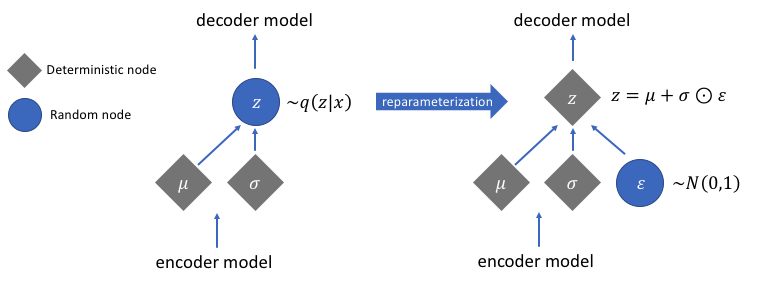
\includegraphics[keepaspectratio]{Generative Model Overview_files/mediabag/reparam-trick.png}}

So the model become

\pandocbounded{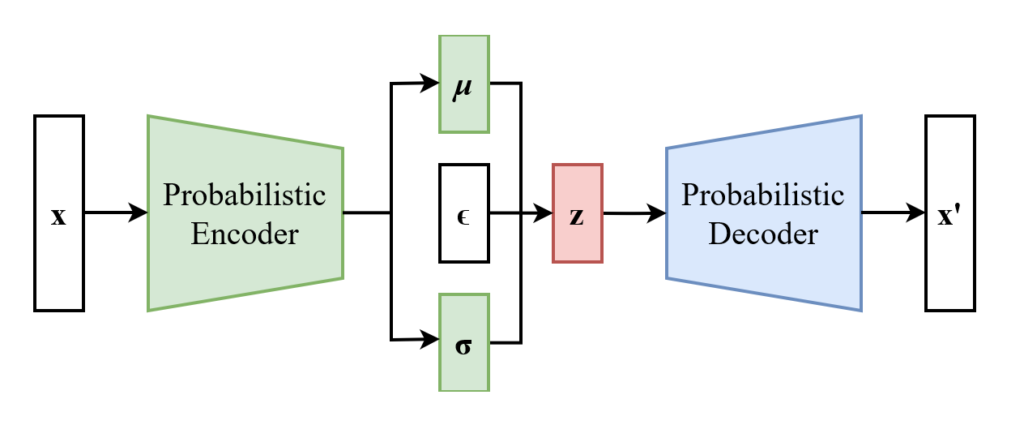
\includegraphics[keepaspectratio]{Generative Model Overview_files/mediabag/vae-reparam.png}}

\section{Generative Adversarial
Networks}\label{generative-adversarial-networks}

GANs are generative models that consist of two neural networks - a
generator \(G\), and a discriminator \(D\)- that complete against each
other in a min-max game framework. The goal is for the generator to
produce data indistinguishable from real samples, while discriminator
tries to distinguish between real and fake(generated) data.

\begin{itemize}
\tightlist
\item
  Generator \(G\): Learns a mapping from random noise \(z \sim p_z(z)\)
  (typically \(z \sim \mathcal{N}(0, I)\) to realistic data sample
  \(x\): \(G(z; \theta_g) : z \mapsto x_{\text{fake}}\)
\item
  Discriminator( \(D\)): Outputs a probability that a given samples
  \(x\) is real (from dataset) rather than fake (from generator):
  \(D(x; \theta_d): x \mapsto [0,1]\)
\end{itemize}

The training of GAN involves solving the following min-max optimization
problem:

\[
\min_{G}\max_{D} V(D, G) = \mathbb{E}_{x \sim p_{\text{data}}(x)}[\log D(x)] + \mathbb{E}_{z \sim p_z(z)}[\log(1 - D(G(z)))]
\]

The training occurs iteratively by alternating steps:

\begin{enumerate}
\def\labelenumi{\arabic{enumi}.}
\tightlist
\item
  Step 1 (Discriminator training): Update discriminator parameters
  \(\theta_d\) to maximize tits objective, thus distinguishing fake from
  real data:
\end{enumerate}

\[
\max_{\theta_d} \mathbb{E}_{x \sim p_{\text{data}}(x)}[\log D(x)] + \mathbb{E}_{z \sim p_z(z)}[\log(1 - D(G(z)))]
\]

\begin{enumerate}
\def\labelenumi{\arabic{enumi}.}
\setcounter{enumi}{1}
\tightlist
\item
  Step 2(Generator training): Update generator parameters \(\theta_g\)
  to minimize the discriminator's success, effectively fooling it:
\end{enumerate}

\[
\min_{\theta_g} \mathbb{E}_{z \sim p_z(z)}[\log(1 - D(G(z)))]
\]

In theory, the training process converges to a \textbf{Nash
Equilibrium}.

\section{Energy-Based Models}\label{energy-based-models}

So far, the generative models modeling the alternative of the
probability of the dataset. In the Energy Based Models, it define
probabilistic models using an energy function, assigning low energy to
configurations(samples) that occur frequently (realistic data points)
and high energy to unlikely configurations. An energy-based model
defines the probability distribution of data \(x\) using an energy
function \(E_\theta[x]\):

\[
p_\theta(x) = \frac{\exp(-E_\theta(x))}{Z(\theta)}
\]

To training from EBMs, one typical is to maximizes the likelihood of
observed data \(p_{\text{data}}(x)\)

\[
\max_\theta \mathbb{E}_{x \sim p_{\text{data}}}(x)[\log p_\theta(x)] = \max_\theta \mathbb{E}_{x \sim p_{\text{data}}}(x)[-E_\theta(x)] - \log Z(\theta)
\]

To Sampling from the Energy Based Model, we using an iterative
approaches such as Markov Chain Monte Carlo(MCMC), especially Langevin
Dynamics.

\section{Flow-Based Models}\label{flow-based-models}

Flow-Based models are generative models that represent complex
probability distributions through invertible transformations of simpler
latent distributions. They explicitly prove tractable likelihood
computation, unlike many other generative models such as GANs and VAEs.

Flow-based models define a generative process by applying an invertible
and differentiable transformation \(f_{\theta}\) (the ``flow'') to a
latent variable \(z\), typically sampled from a simple prior (e.g.,
standard Gaussian):

Given the invertibility of \(f_\theta\) , we can express the likelihood
the of observe data explicitly using the change of variables formula:

\[
p_{X}(x) = p_{Z}(f_{\theta}^{-1}(x)) \left| \det \frac{\partial f_{\theta}^{-1}(x)}{\partial x} \right|
\]

Training Objective of the Flow Model is:

\[
\max_{\theta}\; \mathbb{E}{x \sim p{\text{data}}(x)}\left[ \log p_{X}(x;\theta) \right]
\]

In practice, complex transformations are obtained by composing simpler
invertible transformations
\(f_{\theta}^{(1)}, f_{\theta}^{(2)}, \dots, f_{\theta}^{(K)}\):

\[
f_{\theta}(z) = f_{\theta}^{(K)} \circ f_{\theta}^{(K-1)} \circ \dots \circ f_{\theta}^{(1)}(z)
\]

The determinant of the Jacobian for composed transformations simplifies
as follows:

\[
\log \left| \det \frac{\partial f_{\theta}^{-1}(x)}{\partial x} \right|
= \sum_{i=1}^{K} \log \left| \det \frac{\partial f_{\theta}^{(i)-1}(h_i)}{\partial h_i} \right|
\]

\section{Diffusion Models}\label{diffusion-models}

For more details, please check my this
\href{https://yyzhang2000.github.io/Blog/posts/Generative\%20Model/Diffusion\%20Model.html}{blog}

The Diffusion Models are generative models that learn to reverse a
gradual corruption process applies to data. They gained popularity due
to their impressive results in generating high-quality, diverse samples
across domain such as images, audio, and text. Diffusion models consist
of two processes:

\begin{itemize}
\tightlist
\item
  Forward(Diffusion) Processes:
\end{itemize}

Gradually adds noises to data \(x_0\) over \(T\) timesteps, typically
Gaussian noise:

\[
q(x_t|x_{t-1}) = \mathcal{N}(x_t; \sqrt{1 - \beta_t}x_{t-1}, \beta_t I), \quad t = 1,\dots,T
\]

This form a Markov chain. So the forward distribution can also be
expressed directly in terms of \(x_0\):

\[
q(x_t|x_0) = \mathcal{N}(x_t; \sqrt{\bar{\alpha}_t} x_0, (1 - \bar{\alpha}_t)I)
\]

where
\(\alpha_t = 1 - \beta_t, \quad \bar{\alpha}_t = \prod_{s=1}^{t}\alpha_s\)

\begin{itemize}
\tightlist
\item
  Reverse (Genrative) Process:
\end{itemize}

The generative models learns to reverse this diffusion, gradually
removing noise. It's defined as:

\[
p_\theta(x_{t-1}|x_t) = \mathcal{N}(x_{t-1}; \mu_\theta(x_t, t), \Sigma_\theta(x_t, t))
\]

Diffusion models are trained by maximizing the likelihood of the
observed data. However, in practice, the training often simplifies to a
denoising objective:

\[
L(\theta) = \mathbb{E}{x_0, \epsilon, t}\left[ \|\epsilon - \epsilon\theta(\sqrt{\bar{\alpha}_t} x_0 + \sqrt{1 - \bar{\alpha}_t}\epsilon, t)\|^2 \right]
\]

The Sampling involves starting from pure noise and gradually denoising:

\[
x_{t-1} = \frac{1}{\sqrt{\alpha_t}}\left(x_t - \frac{\beta_t}{\sqrt{1-\bar{\alpha}t}}\epsilon\theta(x_t, t)\right) + \sqrt{\beta_t}\epsilon,\quad \epsilon\sim\mathcal{N}(0, I)
\]

\section{Combining Different Models}\label{combining-different-models}

\subsection{Diffusion Models + VAE}\label{diffusion-models-vae}

\begin{figure}[H]

{\centering \pandocbounded{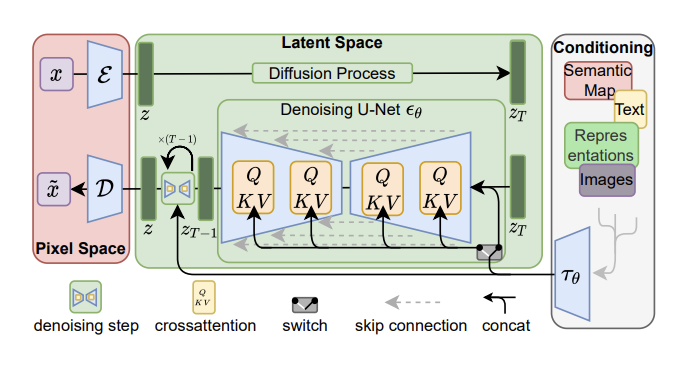
\includegraphics[keepaspectratio]{images/paste-2.png}}

}

\caption{The Architecture of the Stable Diffusion Models (Image Source:
High-Resolution Image Synthesis with Latent Diffusion Models)}

\end{figure}%

One limitation of the diffusion models, it need to go through many steps
on the high-dimensional space. If we can train an model on the lower
dimension and recover it back to the high dimension, than we can speed
up both training and generating process. As proposed in (Rombach et al.
2022), the Latent Diffusion Model is one of those approach. It leverages
latent diffusion techniques, making it computationally efficient and
capable of generating diverse, photorealistic, and detailed visuals from
textual prompts. Widely adopted for its open-source accessibility,
Stable Diffusion enables artists, researchers, and developers to produce
remarkable content easily.

\subsection{Auto-Regressive + VAE}\label{auto-regressive-vae}

\subsection{Auto-Regressive + Flow
Models}\label{auto-regressive-flow-models}

\subsection{Flow Model + VAE}\label{flow-model-vae}

\subsection{Flow Model + GAN}\label{flow-model-gan}

\subsection{VAE + GAN}\label{vae-gan}

As metioned in the paper (Larsen et al. 2016)

\section{Conclusion}\label{conclusion}

In the blog, we has explore go through several generative models. We
explore why we need generative models. For different purposes, we can
different choice of the models. On the other hand, we can combine
different models to get better performance. There are still more room
for the generative models.\\

\phantomsection\label{refs}
\begin{CSLReferences}{1}{0}
\bibitem[\citeproctext]{ref-larsenAutoencodingPixelsUsing2016}
Larsen, Anders Boesen Lindbo, Søren Kaae Sønderby, Hugo Larochelle, and
Ole Winther. 2016. {``Autoencoding Beyond Pixels Using a Learned
Similarity Metric.''} February 10, 2016.
\url{https://doi.org/10.48550/arXiv.1512.09300}.

\bibitem[\citeproctext]{ref-rombachHighResolutionImageSynthesis2022}
Rombach, Robin, Andreas Blattmann, Dominik Lorenz, Patrick Esser, and
Björn Ommer. 2022. {``High-{Resolution Image Synthesis} with {Latent
Diffusion Models}.''} April 13, 2022.
\url{https://doi.org/10.48550/arXiv.2112.10752}.

\end{CSLReferences}




\end{document}
